\chapter{Metodología Experimental y Numérica}
\label{chap:Metodologia}

\section{Introducción}

Habiendo establecido en el Capítulo 2 los fundamentos físicos de la resistencia al avance y las bases teóricas de la mecánica de fluidos, este capítulo detalla la implementación práctica de las herramientas utilizadas en esta tesis. La investigación adopta una estrategia híbrida que vincula ensayos físicos en canal de remolque (EFD) con simulaciones numéricas de alta fidelidad (CFD).

A continuación se describen las instalaciones experimentales del canal de pruebas del LabHiNO, las características geométricas de los modelos construidos y la instrumentación empleada. Posteriormente, se detalla la configuración del modelo numérico en ``OpenFOAM'', especificando el dominio computacional, las condiciones de contorno y los esquemas de discretización utilizados.

\section{Metodología Experimental (EFD)}

Los ensayos experimentales se llevaron a cabo en el canal de remolque de la Universidad de Buenos Aires (UBA), Argentina. Esta campaña tuvo como objetivo principal generar una base de datos de validación confiable para los modelos pesqueros P1, P2 y P3 y comparar los resultados con el buque de referencia KCS.

\subsection{Instalaciones: El Canal de Remolque}

Los ensayos se realizaron en el canal de remolque del LabHiNO. Esta instalación cuenta con un vaso de hormigón rectilíneo con las siguientes dimensiones principales:

\begin{itemize}
    \item \textbf{Longitud:} 72 m
    \item \textbf{Ancho:} 3.6 m
    \item \textbf{Profundidad:} 2.0 m
\end{itemize}

El canal está equipado con un carro dinamométrico capaz de alcanzar una velocidad máxima de 4.0 m/s, lo cual cubre holgadamente el rango de velocidades de Froude requeridas para los modelos analizados en este estudio.

\subsection{Modelos Físicos \label{sec:presentacion_modelos}}

Se fabricaron y ensayaron cuatro modelos a escala, de los cuales tres son pesqueros diseñados por astilleros argentinos y uno un portacontenedores de referencia. Todos fueron acabados con pintura de alto brillo para garantizar una superficie hidráulicamente lisa. A continuación se presentan los mismos.

\subsubsection{Modelo Pesquero 1}
El primer modelo estudiado, de ahora en más \textit{P1}, diseñado por el astillero ``TecnoPesca Argentina'', representa un buque pesquero de baja esbeltez ($L/B < 4$) característico de la flota nacional. El modelo fue construido a escala $\lambda = 20$.

En la Figura \ref{fig:model_tpa}, se presentan las vistas del modelo físico terminado. Se pueden apreciar las marcas de las diferentes secciones, lineas de agua y la disposición de la proa con bulbo. Para asegurar la transición a régimen turbulento de la capa límite y evitar la laminarización del flujo a bajas velocidades, se instalaron estimuladores de turbulencia (alambres cilíndricos de 3 mm de diámetro) a un 5\% de la eslora desde la perpendicular de proa, siguiendo las recomendaciones de la ITTC (Procedimiento 7.5-01-01-01).

\begin{figure}[htpb]
    \centering
    \begin{subfigure}[b]{0.48\textwidth}
        \centering
        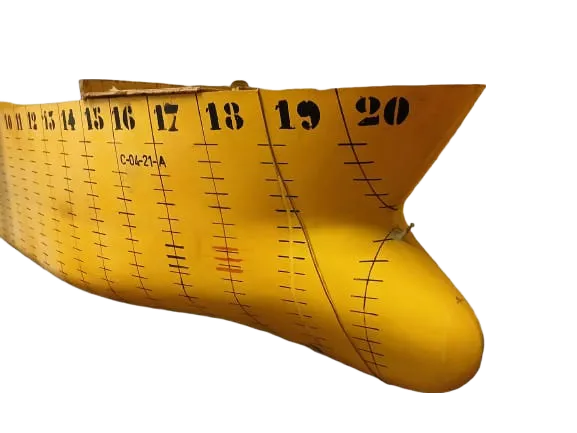
\includegraphics[width=\textwidth]{images/tpa-pers.png}
        \caption{Vista en perspectiva de proa. Se observan las marcas de calado y los estimuladores de turbulencia.}
        \label{fig:tpa_pers}
    \end{subfigure}
    \hfill
    \begin{subfigure}[b]{0.48\textwidth}
        \centering
        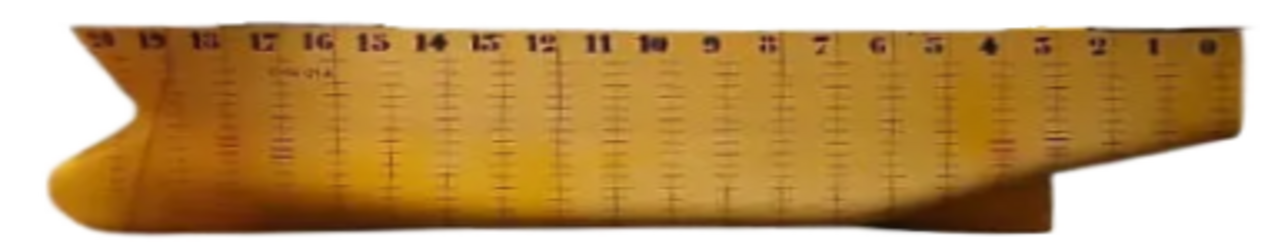
\includegraphics[width=\textwidth]{images/tpa-side.png}
        \caption{Vista de perfil. Geometría de baja esbeltez típica de pesqueros.}
        \label{fig:tpa_side}
    \end{subfigure}
    \caption{Modelo físico del pesquero TPA (Escala 1:20) preparado para ensayos en el LabHiNO.}
    \label{fig:model_tpa}
\end{figure}

El modelo se evaluó en tres condiciones de carga (ligero, medio y pesado) para barrer un rango operativo amplio y analizar la sensibilidad del factor de forma al calado. Las áreas transversales medias del modelo representaron el 1\%, 1.1\% y 1.2\% del área transversal del tanque para las condiciones de carga ligera, media y pesada, respectivamente.

La Tabla~\ref{tab:main_param_p1} resume las características geométricas y dinámicas del buque pesquero en escala real (T1) y del modelo en las tres condiciones de calado ensayadas (T1, T2 y T3).

\begin{table}[H]
\caption{Características principales del pesquero P1 en escala real y del modelo en tres condiciones de calado.}
\centering
\begin{tabularx}{\textwidth}{lllllll}
\toprule
\textbf{Característica}&\textbf{Símbolo}&\textbf{Unidad}&\textbf{Escala Real }&\textbf{Modelo} & \textbf{Modelo} & \textbf{Modelo}\\
 &  & & \textbf{T1} & \textbf{T1}& \textbf{T2} & \textbf{T3}\\
\midrule
Escala del modelo & $\lambda$ & {[}-{]} & - & 20 & 20 & 20\\
Eslora en flotación & L$_{WL}$ & {[}m{]} & 32.68 & 1.634 & 1.662 & 1.641\\
Eslora total sumergida & L$_{OS}$ & {[}m{]} & 34.795 & 1.670 & 1.740 & 1.740\\
Manga & B & {[}m{]} & 9.28 & 0.464 & 0.464 & 0.464\\
Calado & T & {[}m{]} & 3.30 & 0.165 & 0.180 & 0.195\\
Volumen de desplazamiento & V & {[}m$^3${]} & 599.40 & 0.075 & 0.085 & 0.095\\
Área de superficie mojada & S & {[}m$^2${]} & 392.67 & 0.982 & 1.058 & 1.124\\
Coeficiente de bloque & C$_B$ & {[}-{]} & 0.60 & 0.60 & 0.61 & 0.64\\
Desplazamiento (masa) & $\Delta$ & {[}t{]} & - & 75.0 & 85.0 & 95.0\\
\bottomrule
\end{tabularx}
\label{tab:main_param_p1}
\end{table}

\subsubsection{Modelo Pesquero 2}
El tercer pesquero analizado, de ahora en más P3, fue diseñado y construido por el Astillero Naval Federico Contessi y Cía. S.A. El modelo fue construido a escala $\lambda = 10$ y ensayado en una sola condición de calado. La Tabla~\ref{tab:main_param_p3} resume sus características principales.

\begin{table}[H]
\caption{Características principales del pesquero P3.}
\centering
\begin{tabularx}{\textwidth}{lllll}
\toprule
\textbf{Característica}&\textbf{Símbolo}&\textbf{Unidad} & \textbf{Escala Real} & \textbf{Modelo (T1)}\\
 &  &  & (Buque) &  \\
\midrule
Escala del modelo & $\lambda$ & {[}-{]} & - & 10 \\
Eslora en flotación& L$_{WL}$ & {[}m{]} & 25.100 & 2.510 \\
Eslora total sumergida & L$_{OS}$ & {[}m{]} & 26.580 & 2.658 \\
Manga & B & {[}m{]} & 7.800 & 0.780 \\
Calado & T & {[}m{]} & 3.460 & 0.346 \\
Volumen de desplazamiento & V & {[}m$^3${]} & 387.265 & 0.387 \\
Área de superficie mojada & S & {[}m$^2${]} & 292.000 & 2.920 \\
Coeficiente de bloque & C$_B$ & {[}-{]} & 0.577 & 0.571 \\
Desplazamiento (masa) & $\Delta$ & {[}t{]} & 397.295 & 387.0 \\
\bottomrule
\end{tabularx}
\label{tab:main_param_p2}
\end{table}

\subsubsection{Modelo Pesquero 3}
El segundo pesquero analizado, de ahora en más P2, fue diseñado y construido por el astillero JPA S.A. El modelo fue construido a escala $\lambda = 13$ y ensayado en una sola condición de calado. La Tabla~\ref{tab:main_param_p2} resume sus características principales.

\begin{table}[H]
\caption{Características principales del pesquero P2.}
\centering
\begin{tabularx}{\textwidth}{lllll}
\toprule
\textbf{Característica}&\textbf{Símbolo}&\textbf{Unidad} & \textbf{Escala Real} & \textbf{Modelo (T1)}\\
 &  &  & (Buque) &  \\
\midrule
Escala del modelo & $\lambda$ & {[}-{]} & - & 13 \\
Eslora en flotación & L$_{WL}$ & {[}m{]} & 22.050 & 1.696 \\
Eslora total sumergida & L$_{OS}$ & {[}m{]} & 22.282 & 1.714 \\
Manga & B & {[}m{]} & 7.800 & 0.600 \\
Calado & T & {[}m{]} & 3.050 & 0.235 \\
Volumen de desplazamiento & V & {[}m$^3${]} & 320.070 & 0.146 \\
Área de superficie mojada & S & {[}m$^2${]} & 240.964 & 1.426 \\
Coeficiente de bloque & C$_B$ & {[}-{]} & 0.643 & 0.608 \\
Desplazamiento (masa) & $\Delta$ & {[}t{]} & 328.360 & 146.0 \\
\bottomrule
\end{tabularx}
\label{tab:main_param_p3}
\end{table}


\subsubsection{Modelo de Referencia KCS}
Con el fin de complementar el análisis mediante la inclusión de un buque completamente diferente a los pesqueros, se construyó un modelo del portacontenedores ``KRISO Container Ship'' (KCS) a escala $\lambda = 79$. Este buque de alto valor referencial presenta características hidrodinámicas marcadamente distintas: una esbeltez muy superior (relación $L/B \approx 7.1$ vs. $L/B \approx 2.8$–$3.5$ para los pesqueros), una popa afinada con transición suave de cuerpo paralelo a codaste en contraste con la popa llena característica de los pesqueros, y la ausencia de dormido significativo frente al dormido pronunciado de los buques pesqueros. La Tabla~\ref{tab:main_param_kcs} resume sus características principales.

La Figura \ref{fig:model_kcs} muestra el modelo KCS, permitiendo comparar visualmente la geometría esbelta y refinada de este portacontenedores con la forma llena y robusta de los pesqueros argentinos. 

\begin{table}[H]
\caption{Características principales del portacontenedores KCS.}
\centering
\begin{tabularx}{\textwidth}{lllll}
\toprule
\textbf{Característica}&\textbf{Símbolo}&\textbf{Unidad} & \textbf{Escala Real} & \textbf{Modelo}\\
 &  &  & (Buque) & (T1) \\
\midrule
Escala del modelo & $\lambda$ & {[}-{]} & - & 79 \\
Eslora en flotación & L$_{WL}$ & {[}m{]} & 230.000 & 2.911 \\
Eslora total sumergida & L$_{OS}$ & {[}m{]} & 232.500 & 2.943 \\
Manga & B & {[}m{]} & 32.200 & 0.408 \\
Calado & T & {[}m{]} & 10.800 & 0.137 \\
Volumen de desplazamiento & V & {[}m$^3${]} & 52030.000 & 0.106 \\
Área de superficie mojada & S & {[}m$^2${]} & 9530.000 & 1.527 \\
Coeficiente de bloque & C$_B$ & {[}-{]} & 0.595 & 0.653 \\
Desplazamiento (masa) & $\Delta$ & {[}t{]} & 51925.940 & 105.318 \\
\bottomrule
\end{tabularx}
\label{tab:main_param_kcs}
\end{table}

\subsection{Instrumentación y Adquisición de Datos}

La medición de la resistencia total al avance ($R_T$) se realizó mediante una celda de carga de un solo componente marca \textbf{Kempf \& Remmers modelo R 47}. El transductor, diseñado para una carga a escala completa de $\pm 100$ N, posee una sensibilidad de aproximadamente $\pm 1$ mV/V de voltaje de alimentación.

El montaje del modelo al carro dinamométrico se realizó vinculándolo a la celda de carga de manera tal que se restringieron los movimientos de avance (velocidad constante impuesta por el carro), deriva, guiñada y rolido. El sistema permitió que el modelo quedara \textbf{libre a cabeceo (``trim'') y hundimiento (``sinkage'')}, conforme a los estándares para ensayos de resistencia al avance.

El sistema de adquisición de datos se configuró con los siguientes parámetros:
\begin{itemize}
    \item \textbf{Frecuencia de muestreo:} 200 Hz, permitiendo capturar la dinámica transitoria y las fluctuaciones.
    \item \textbf{Post-procesamiento:} Se aplicó un filtro paso bajo de 4 Hz a la señal para eliminar el ruido eléctrico y vibraciones mecánicas de alta frecuencia.
\end{itemize}

\subsection{Procedimiento de Ensayo y Análisis de Incertidumbre}

Se siguió el procedimiento estándar para ensayos de resistencia según la ITTC (7.5-02-02-01).

Dado que el modelo ocupa una fracción del volumen del canal, la presencia de las paredes y el fondo acelera el flujo alrededor del casco (efecto de bloqueo). Aunque las relaciones de área transversal fueron bajas ($1\% - 1.2\%$), se aplicó la \textbf{corrección de bloqueo de Schuster} a los resultados experimentales para garantizar la consistencia con la condición de aguas ilimitadas, de acuerdo con el procedimiento de la ITTC \cite{ITTC_resistance}.

\subsubsection*{Metodología de Análisis de Incertidumbre}
\label{sec:analisis_incertidumbre_general}

El análisis de incertidumbre para la medición de resistencia requiere la consideración exhaustiva de todas las fuentes significativas de error. El presente análisis sigue las directrices establecidas por la ITTC \cite{ITTC_uncertainty}, combinando componentes de incertidumbre mediante el método de la Raíz de la Suma de los Cuadrados (RSS, ``Root Sum Squares'').

\paragraph{Componentes de incertidumbre consideradas}

La resistencia total medida es función de múltiples variables independientes. Las incertidumbres se propagaron a través de cada una de estas dependencias:

\begin{itemize}
    \item \textbf{Geometría del casco:} La incertidumbre en el desplazamiento y la superficie mojada se cuantificó midiendo el lastre del modelo con una balanza de brazo portátil. Asumiendo que la incertidumbre geométrica no afecta significativamente el coeficiente de resistencia residual, la propagación ocurre a través de la superficie mojada y la eslora representativa. La incertidumbre estándar en la masa de desplazamiento constituye la fuente primaria para esta componente.

    \item \textbf{Velocidad de remolque:} Se consideró el límite de sesgo (``bias limit'') del carro dinamométrico. Este error se propaga a la medición de resistencia a través de la presión dinámica $q = \tfrac{1}{2}\rho V^2$ y en consecuencia al número de Reynolds. Para el rango operativo del LabHiNO, la precisión adoptada refleja la capacidad de control del sistema de remolque.

    \item \textbf{Temperatura del agua:} Dado que la viscosidad cinemática $\nu$ es fuertemente dependiente de la temperatura, variaciones de la misma afectan directamente al número de Reynolds $Re = \tfrac{V \cdot L}{\nu}$ y a la componente friccional de la resistencia. Se monitoreó la temperatura durante todos los ensayos. Las variaciones observadas se mantuvieron por debajo de $0.5\,^\circ$C, lo que implica variaciones en la viscosidad del orden del 2\% en el rango de interés.

    \item \textbf{Calibración del dinamómetro:} El transductor Kempf \& Remmers R47 se calibró antes y después de cada sesión de ensayo utilizando pesas patrón certificadas. Se ajustó una recta a los datos de calibración mediante regresión lineal, y la desviación estándar de esta regresión se adoptó como la incertidumbre estándar de calibración. Las pesas patrón empleadas fueron de precisión suficientemente alta como para considerarse su contribución despreciable.

    \item \textbf{Adquisición de datos (DAS):} La señal del dinamómetro se adquirió a frecuencia de muestreo de 200 Hz y fue filtrada mediante un filtro pasa bajos de 4 Hz antes de ingresar al sistema de adquisición. El promedio de cada ensayo se calculó sobre la historia temporal durante intervalos de al menos 10 segundos. La incertidumbre estándar del promedio temporal fue evaluada para cada repetición, resultando en valores entre $0.0007\%$ y $0.003\%$. Estos valores resultan despreciables en comparación con otras fuentes de error, confirmando la estabilidad del sistema de adquisición.

    \item \textbf{Repetibilidad:} Se realizaron múltiples repeticiones de cada ensayo a una misma velocidad. La media aritmética de estas repeticiones se adoptó como la mejor estimación de la resistencia. La incertidumbre estándar de la media de $N$ mediciones repetidas se estimó de acuerdo con el procedimiento de la ITTC, considerando tanto la dispersión entre repeticiones como el número de replicaciones.
\end{itemize}

\paragraph{Combinación de componentes mediante RSS}

Una vez estimadas todas las componentes individuales de incertidumbre, la incertidumbre combinada se calculó mediante:

\begin{equation}
u_c = \sqrt{u_1^2 + u_2^2 + \cdots + u_n^2}.
\end{equation}

La incertidumbre expandida, correspondiente a un nivel de confianza del 95\%, se obtuvo multiplicando la incertidumbre combinada por el factor de cobertura $k = 2$.

\paragraph{Comportamiento característico con el número de Froude}

Un hallazgo importante del análisis de incertidumbre es su dependencia funcional con la velocidad de remolque (o equivalentemente, con el número de Froude). A bajos números de Froude, la resistencia total es pequeña y la relación señal-ruido del dinamómetro se deteriora, amplificando la incertidumbre relativa. En este régimen, la calibración del dinamómetro y la dispersión entre repeticiones constituyen las fuentes dominantes. A medida que aumenta la velocidad, la resistencia total crece y la incertidumbre relativa disminuye, mejorando la relación señal-ruido.

Este comportamiento es consistente con lo esperado para ensayos de remolque y debe ser considerado en la comparación cuantitativa con resultados numéricos.

Los valores cuantitativos finales de la incertidumbre combinada y expandida para las distintas velocidades de ensayo específicas se presentan en detalle junto con los resultados experimentales en el Capítulo~\ref{cap:resistencia_factor_de_forma}.

\section{Procedimiento de extrapolación modelo--buque}
\label{sec:prediccion_potencia}

Una vez obtenida la resistencia del modelo mediante ensayos experimentales
o simulaciones numéricas, el paso siguiente consiste en extrapolar estos
resultados a escala buque. El procedimiento estándar recomendado por la
ITTC \citep{ITTC_Performance_prediction} se basa en la descomposición de
la resistencia total en sus componentes viscosa y de formación de olas,
escalando cada una de manera independiente.

El coeficiente de resistencia total del modelo se descompone como:
%
\begin{equation}
    C_{TM} = (1 + k_M)\,C_{FM0} + C_W ,
\end{equation}
%
donde $C_{FM0}$ es el coeficiente de fricción del modelo calculado mediante
la línea ITTC-57 (Sección~\ref{sec:ITTC57}) al número de Reynolds del modelo, $k_M$ es el factor de forma a escala modelo, determinado por el método de Prohaska como propone la ITTC \citep{ITTC_Performance_prediction}, por métodos empíricos, o según los métodos descritos en el Capítulo~\ref{cap:resistencia_factor_de_forma}, y $C_W$ es el coeficiente de resistencia por formación de olas, obtenido como residuo:
%
\begin{equation}\label{eq:CW_residuo}
    C_W = C_{TM} - (1+k_M)\,C_{FM0} .
\end{equation}
%
La hipótesis central del método es que $C_W$, así determinado, es
independiente del número de Reynolds y escala directamente con el número de
Froude. Bajo este supuesto, la resistencia total a escala buque se estima
como:
%
\begin{equation}\label{eq:CTS}
    C_{TS} = (1 + k_S)\,C_{FS0} + C_W + \Delta C_F + C_A + C_{AAS} ,
\end{equation}
%
\footnote{La corrección por rugosidad corresponde a la formulación de Townsin
y Dey, incorporada por la ITTC en 1990:
$\Delta C_F = 0.044\big[(k_s/L_{WL})^{1/3} - 10\,Re_S^{-1/3}\big] + 0.000125$,
donde $k_s$ es la altura de rugosidad equivalente (adoptada como
$k_s = 150\,\mu\text{m}$ en ausencia de mediciones directas) y $Re_S$ el
número de Reynolds del buque. El coeficiente de correlación, separado de la
rugosidad por el 19.\textsuperscript{o} ITTC, se calcula como
$C_A = (5.68 - 0.6\log_{10} Re_S)\times 10^{-3}$. Esta separación
reemplaza la formulación combinada original de Bowden y Davison
\citep{ITTC_Performance_prediction}.}

donde $C_{FS0}$ es el coeficiente de fricción del buque calculado mediante la línea ITTC-57 al número de Reynolds del buque, $k_S$ es el factor de forma a escala buque, $\Delta C_F$ es la corrección por rugosidad de la superficie, $C_A$ es el coeficiente de correlación modelo--buque y $C_{AAS}$ es el coeficiente de resistencia aerodinámica de la obra muerta, todos evaluados según las formulaciones recomendadas por la ITTC
\citep{ITTC_Performance_prediction}.

Conviene subrayar la estructura de las Ecuaciones~\eqref{eq:CW_residuo}
y~\eqref{eq:CTS}: la resistencia por olas $C_W$ se calcula con el factor de
forma de modelo $k_M$ y se traslada sin modificación a la escala buque,
mientras que la componente viscosa se escala con el factor de forma de buque $k_S$. El método estándar de la ITTC asume $k_S = k_M$, es decir, un factor de forma independiente de la escala, con lo que ambas ecuaciones se reducen al procedimiento clásico de un único factor de forma. Cuando, en cambio, se admite $k_S \neq k_M$, la formulación coincide con el método de dos factores de forma ($2k$) de \citet{korkmaz_wetted_transom}, en el que la componente viscosa se corrige por efectos de escala sin alterar la residual. Como se analiza en profundidad en el Capítulo~\ref{cap:resistencia_factor_de_forma}, la hipótesis $k_S = k_M$ no se cumple para los pesqueros estudiados en esta tesis, lo que hace necesario el uso de la formulación de dos factores de forma.

La resistencia total del buque y la potencia efectiva se obtienen como:
%
\begin{equation}
    R_{TS} = \tfrac{1}{2}\,\rho\,V_S^2\,S_S\,C_{TS},
\end{equation}
%
\begin{equation}
    P_{ES} = R_{TS}\,V_S,
\end{equation}
%
donde $\rho$ es la densidad del agua, $V_S$ la velocidad del buque y $S_S$
la superficie mojada a escala buque.

\section{Metodología Numérica (CFD)}

Las simulaciones numéricas se realizaron utilizando el código de código abierto \textbf{OpenFOAM} (versión 11), basado en el Método de Volúmenes Finitos (FVM).

\subsection{Dominio Computacional y Mallado}

Se definió un dominio computacional rectangular prismático dimensionado para evitar la reflexión de olas.
\begin{itemize}
    \item \textbf{Entrada (Inlet):} Ubicada a $1.5 L_{pp}$ a proa del modelo.
    \item \textbf{Salida (Outlet):} Ubicada a $2.5 L_{pp}$ a popa.
    \item \textbf{Límites laterales y fondo:} Ubicados a distancia suficiente para simular aguas profundas.
\end{itemize}

El mallado se generó con \texttt{snappyHexMesh}, utilizando una estructura predominantemente hexaédrica no estructurada con refinamientos locales en la superficie libre y la estela, e inserción de capas de prismas en la superficie del casco para resolver la capa límite ($y^+$ controlado).

\subsection{Configuración de los Casos de Estudio}

Se emplearon dos configuraciones de simulación distintas. A continuación se detallan las condiciones de contorno específicas seleccionadas para garantizar la estabilidad y conservación de masa en el dominio.

\subsubsection{Simulación con Superficie Libre}
Esta configuración replica el ensayo de canal para obtener la resistencia total ($R_T$) y el campo de olas.

\begin{itemize}
    \item \textbf{Solucionador:} \texttt{interFoam} (VoF con compresión de interfaz MULES).
    \item \textbf{Algoritmo:} PIMPLE (híbrido PISO-SIMPLE).
\end{itemize}

La Figura \ref{fig:dominio_metodologia} esquematiza el dominio computacional utilizado, mostrando la disposición de las condiciones de contorno.

\begin{figure}[htpb]
    \centering
    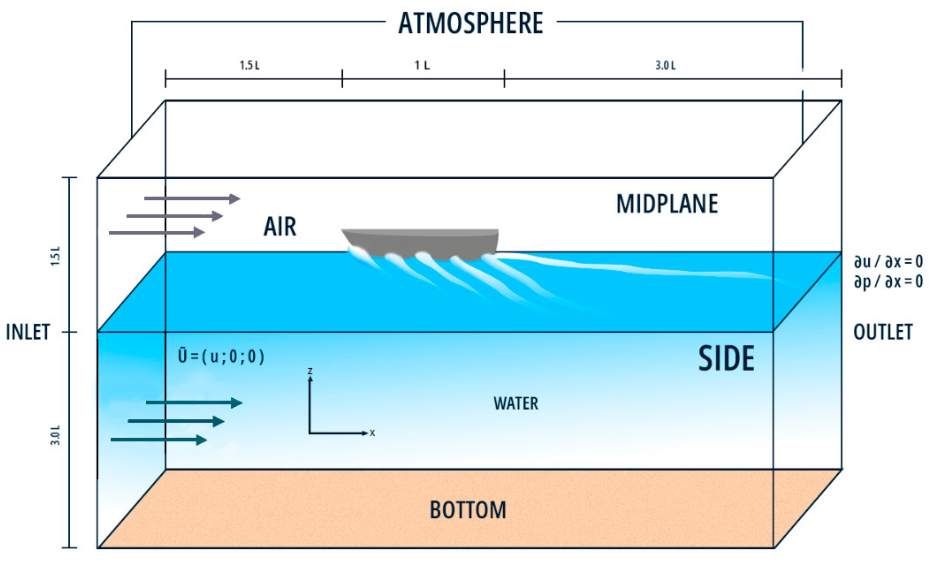
\includegraphics[width=0.6\textwidth]{images/domain.png}
    \caption{Dominio computacional y condiciones de contorno para las simulaciones de resistencia con superficie libre.}
    \label{fig:dominio_metodologia}
\end{figure}

Las condiciones de borde específicas se resumen en la Tabla \ref{tab:bc_setup}.

\begin{table}[H]
\centering
\caption{Condiciones de borde específicas para las simulaciones con superficie libre (VoF).}
\label{tab:bc_setup}
\small
\begin{tabular}{lcccc}
\toprule
\textbf{Variable} & \textbf{Entrada} & \textbf{Salida} & \textbf{Atmósfera} & \textbf{Casco} \\
\midrule
$U$ & FV & OPMV & PIOV & MWV \\
$p_{rgh}$ & FFP & ZG & TP & FFP \\
$\alpha_{water}$ & FV & VHFR & IO & ZG \\
$k$ & FV & IO & IO & kLRWF \\
$\omega$ & FV & IO & IO & oWF \\
$\nu_t$ & calc. & calc. & calc. & nutkWF \\
\bottomrule
\end{tabular}
\end{table}

\noindent\textbf{Definición de condiciones de borde:}
\begin{itemize}
    \item \textbf{FV} (\texttt{fixedValue}): Valor fijo.
    \item \textbf{ZG} (\texttt{zeroGradient}): Gradiente nulo.
    \item \textbf{IO} (\texttt{inletOutlet}): Permite flujo reverso.
    \item \textbf{FFP} (\texttt{fixedFluxPressure}): Ajusta gradiente de presión por flujo másico.
    \item \textbf{OPMV} (\texttt{outletPhaseMeanVelocity}): Velocidad media de fase en salida.
    \item \textbf{PIOV} (\texttt{pressureInletOutletVelocity}): Velocidad dependiente de presión.
    \item \textbf{TP} (\texttt{totalPressure}): Presión total fija.
    \item \textbf{MWV} (\texttt{movingWallVelocity}): Velocidad de pared (cero relativo).
    \item \textbf{VHFR} (\texttt{variableHeightFlowRate}): Altura variable de superficie libre.
    \item \textbf{kLRWF} / \textbf{oWF} / \textbf{nutkWF}: Funciones de pared para turbulencia.
\end{itemize}

\subsubsection{Simulación de Doble Cuerpo}\label{sec:doble_cuerpo}

Esta configuración se utiliza exclusivamente para aislar la resistencia viscosa ($R_V$) y determinar el factor de forma $(1+k)$. El término ``Doble Cuerpo'' hace referencia al concepto aerodinámico de reflejar el casco sumergido respecto al plano de flotación, generando un cuerpo equivalente completamente sumergido en un fluido infinito.

\paragraph{Fundamento Físico y Dominio}
En esta aproximación, la superficie libre se sustituye por una condición de \textbf{tapa rígida sin fricción} (``frictionless rigid lid''). Geométricamente, el dominio se trunca en la línea de flotación estática ($z=0$), tal como se ilustra en la Figura \ref{fig:double_body_domain}.

\begin{figure}[htpb]
    \centering
    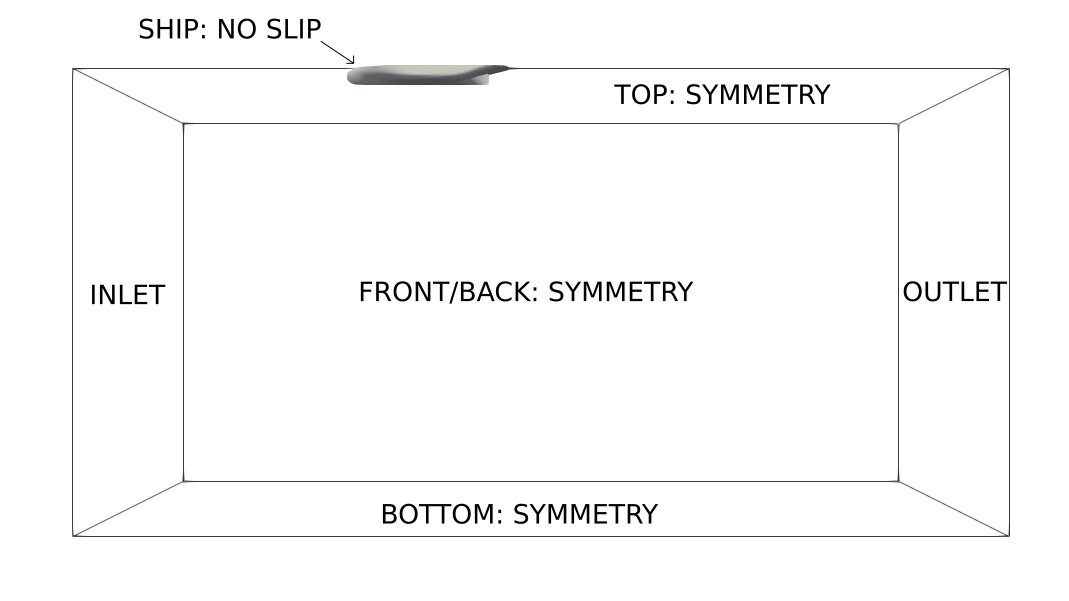
\includegraphics[width=0.6\textwidth]{images/esquema_malla}
    \caption{Dominio reducido para simulación sin superficie libre (Doble Cuerpo), mostrando la condición de simetría en el plano de flotación.}
    \label{fig:double_body_domain}
\end{figure}

\begin{itemize}
    \item \textbf{Plano de Simetría:} La frontera superior del dominio se define como un \texttt{symmetryPlane}. Matemáticamente, esto impone dos restricciones fundamentales:
    \begin{enumerate}
        \item Flujo impenetrable: La componente normal de la velocidad es nula ($\mathbf{v} \cdot \mathbf{n} = 0$).
        \item Cero esfuerzo cortante: El gradiente normal de la velocidad tangencial es nulo ($\partial \mathbf{v}_t / \partial n = 0$).
    \end{enumerate}
    Esta configuración elimina la generación de olas ($R_W = 0$) y la energía potencial gravitatoria, permitiendo que la presión calculada corresponda únicamente a la presión hidrodinámica viscosa.
\end{itemize}

\paragraph{Ventajas del Mallado}
Al eliminar la necesidad de capturar la interfase aire-agua, se prescinde del refinamiento de malla vertical en la zona de superficie libre. Esto permite concentrar la densidad de celdas en la capa límite y, crucialmente, en la \textbf{estela viscosa} y la zona de recirculación del espejo de popa (``transom''), optimizando el costo computacional global frente a las simulaciones VoF.

\paragraph{Configuración Numérica (PIMPLE)}
A diferencia de los enfoques estacionarios clásicos, en este trabajo se utilizó un solucionador transitorio (\textbf{\texttt{pimpleFoam}}) para resolver las ecuaciones RANS monofásicas.
\begin{itemize}
    \item \textbf{Justificación:} Se optó por la resolución transitoria para garantizar la estabilidad numérica frente a desprendimientos de flujo complejos y oscilantes en la zona del espejo de popa, los cuales suelen dificultar la convergencia de solucionadores estacionarios (tipo SIMPLE).
    \item \textbf{Algoritmo:} Se utilizó el algoritmo PIMPLE, que permite utilizar pasos de tiempo grandes ($Co_{max} > 1$) manteniendo la estabilidad mediante correcciones externas en cada paso de tiempo.
    \item \textbf{Convergencia:} La simulación se ejecutó hasta alcanzar un estado cuasi-estacionario donde las fuerzas hidrodinámicas oscilan en torno a un valor medio constante.
\end{itemize}

\paragraph{Cálculo del Factor de Forma}
La resistencia viscosa total $R_V$, compuesta por la fricción tangencial $R_F$
y la presión viscosa $R_{PV}$, se obtuvo promediando la señal de resistencia
en el intervalo de tiempo convergido. El factor de forma se determina como:
%
\begin{equation}
    (1+k) = \frac{C_V}{C_{F0}},
\end{equation}
%
donde $C_V = C_F + C_{PV}$ es el coeficiente de resistencia viscosa
obtenido de la simulación de doble cuerpo y $C_{F0}$ es el coeficiente
de la línea ITTC-57, definido en la Sección~\ref{sec:ITTC57}. Se adopta la
línea ITTC-57 como referencia de $C_{F0}$ para preservar la coherencia con
los factores de correlación históricos, siguiendo la recomendación de la
ITTC \citep{ITTC_Combined_2021}. El valor del factor de forma resultante
depende, no obstante, de la línea de fricción elegida, y estudios recientes
que emplean líneas de fricción numéricas \citep{quintuna2023} obtienen
factores de forma sistemáticamente mayores y menos dependientes de la escala,
por lo que los valores aquí reportados deben interpretarse siempre en
relación con la línea de referencia empleada.

\subsection{Modelado de la Turbulencia: Modelo $k$--$\omega$ SST}
\label{sec:metodo_SST}

Para el cierre del sistema de ecuaciones RANS, se seleccionó el modelo \textbf{$k$--$\omega$ SST (Shear Stress Transport)}, desarrollado en \citet{Menter1994}. Este modelo se ha convertido en el estándar de la industria naval debido a su capacidad para predecir con mayor precisión el inicio y la magnitud de la separación del flujo bajo gradientes de presión adversos, una característica crítica en la hidrodinámica de popas de buques pesqueros.

El modelo SST es una formulación híbrida de dos ecuaciones que resuelve el transporte de la energía cinética turbulenta ($k$) y la tasa específica de disipación ($\omega$). Su principal ventaja radica en la combinación zonal: utiliza la robusta formulación original $k$--$\omega$ de Wilcox en la región cercana a la pared (capa límite) y conmuta al modelo estándar $k$--$\varepsilon$ en la región de flujo libre. Esta estrategia evita la conocida sensibilidad del modelo $k$--$\omega$ a las condiciones de turbulencia en el borde de entrada (``freestream sensitivity'').

Las ecuaciones de transporte para $k$ y $\omega$ en el modelo SST son:

\begin{equation}
    \frac{\partial (\rho k)}{\partial t} + \frac{\partial (\rho U_i k)}{\partial x_i} = \tilde{P}_k - \beta^* \rho k \omega + \frac{\partial}{\partial x_i} \left[ (\mu + \sigma_k \mu_t) \frac{\partial k}{\partial x_i} \right],
\end{equation}

\begin{equation}
    \frac{\partial (\rho \omega)}{\partial t} + \frac{\partial (\rho U_i \omega)}{\partial x_i} = \alpha \rho S^2 - \beta \rho \omega^2 + \frac{\partial}{\partial x_i} \left[ (\mu + \sigma_\omega \mu_t) \frac{\partial \omega}{\partial x_i} \right] + 2(1-F_1) \rho \sigma_{\omega 2} \frac{1}{\omega} \frac{\partial k}{\partial x_i} \frac{\partial \omega}{\partial x_i},
\end{equation}

donde $\rho$ es la densidad del fluido, $U_i$ la componente $i$ de la
velocidad, $\mu$ la viscosidad dinámica molecular, $\mu_t$ la viscosidad
turbulenta dinámica, $\tilde{P}_k$ el término de producción limitado de
turbulencia, $F_1$ la función de mezcla del modelo SST, y $\sigma_k$,
$\sigma_\omega$, $\beta$, $\beta^*$ y $\alpha$ son coeficientes del modelo
interpolados mediante $F_1$ entre los valores de los modelos
$k$--$\omega$ y $k$--$\varepsilon$.

El último término de la ecuación de $\omega$ representa la \textbf{difusión cruzada} (``cross-diffusion''), que se activa únicamente en la zona de flujo libre ($F_1 \to 0$), permitiendo transformar matemáticamente el modelo $k$--$\varepsilon$ en una formulación basada en $\omega$.

\paragraph{Definición de la Viscosidad Turbulenta}
La diferencia fundamental del modelo SST respecto a los modelos estándar radica en la definición de la viscosidad turbulenta ($\nu_t$). En las capas límite sujetas a gradientes de presión adversos, la hipótesis estándar de Boussinesq sobreestima el esfuerzo cortante de Reynolds, lo que conduce a una predicción tardía de la separación del flujo.

Para corregir esto, Menter introdujo un limitador basado en la hipótesis de Bradshaw, que establece que el esfuerzo cortante es proporcional a la energía cinética turbulenta en la mayor parte de la capa límite. La viscosidad turbulenta se calcula como:

\begin{equation}
    \nu_t = \frac{a_1 k}{\max(a_1 \omega, S F_2)},
\end{equation}

donde:
\begin{itemize}
    \item $S = \sqrt{2 S_{ij} S_{ij}}$ es la magnitud del invariante de la tasa de deformación, con $S_{ij} = \tfrac{1}{2}(\partial U_i/\partial x_j + \partial U_j/\partial x_i)$ el tensor de tasa de deformación.
    \item $a_1 = 0.31$ es una constante empírica (coeficiente de estructura de Bradshaw).
    \item $F_2$ es una segunda función de mezcla que restringe el limitador a la capa límite.
\end{itemize}

Esta formulación asegura que $\nu_t$ no crezca excesivamente en zonas de alta deformación y baja vorticidad, permitiendo capturar correctamente la estructura de la estela y los vórtices en la popa del buque.

\paragraph{Tratamiento de Pared}
{\sloppy
En las superficies del casco, se emplearon condiciones de borde tipo función de pared adaptativa disponibles en ``OpenFOAM'' (\texttt{kLowReWallFunction}, \texttt{omegaWallFunction}). Estas condiciones permiten una transición continua entre la integración directa de las ecuaciones hasta la pared (cuando la malla es fina, $y^+ \approx 1$) y el uso de leyes de pared logarítmicas (cuando $y^+ > 30$), asegurando la robustez de la solución independientemente de las variaciones locales de la calidad de la malla.
\par}

\section{Metodología Numérica para Hélices en Aguas Abiertas}
\label{sec:metodologia_helices}

A diferencia de las simulaciones de resistencia del casco descriptas en la sección
anterior, las simulaciones de hélices en aguas abiertas se resuelven en un marco de
referencia solidario a la rotación del propulsor, sin superficie libre. Con el
objetivo de evaluar la robustez de las predicciones frente a la elección del código
de cálculo, este tipo de simulaciones se realizó en paralelo con dos solvers RANS de
naturaleza distinta --StarCCM+ (comercial, solver acoplado) y OpenFOAM (código
abierto, solver segregado)-- cuya configuración específica se detalla a
continuación. Los casos de estudio particulares (geometría de la hélice, rango de
$Re_n$ o $Re_c$ explorado, niveles de intensidad turbulenta ensayados) se presentan en
el Capítulo~\ref{chap:helices} junto con los resultados.

En ambos códigos se emplearon los mismos dos modelos de turbulencia introducidos en la
Sección~\ref{sec:metodo_SST}: el modelo $k$--$\omega$ SST completamente turbulento
como referencia, y el modelo de transición SST-LM
($\gamma$--$\widetilde{Re}_{\theta t}$) de \citet{langtry2009}, que resuelve dos
ecuaciones de transporte adicionales para la intermitencia $\gamma$ y el número de
Reynolds de inicio de transición $\widetilde{Re}_{\theta t}$, acopladas al modelo SST
base.

\subsection{Configuración en StarCCM+}
\label{sec:metodologia_helices_starccm}

Las simulaciones se resuelven en marco de referencia en rotación, empleando las
ecuaciones RANS estacionarias. El dominio y el mallado específicos de cada caso
(dimensiones, densidad de celdas, tratamiento de capa límite) se detallan junto con
cada campaña de simulaciones en el Capítulo~\ref{chap:helices}.

\subsection{Configuración en OpenFOAM}
\label{sec:metodologia_helices_openfoam}

Las simulaciones se realizaron con \textbf{OpenFOAM~8}, empleando el solver
estacionario \texttt{simpleFoam} (algoritmo SIMPLE) sobre un dominio reducido de
$90^\circ$ que modela una única pala, con la periodicidad impuesta mediante una
interfaz de malla móvil (AMI) y el efecto de la rotación incorporado a través de la
formulación de Marco de Referencia Múltiple (MRF). El modelo SST-LM se implementó
utilizando la formulación \texttt{kOmegaSSTLM} disponible de forma nativa en
OpenFOAM~8.

La malla se generó íntegramente dentro del entorno OpenFOAM, combinando
\texttt{cfMesh} para la discretización de la geometría base y \texttt{snappyHexMesh}
para la inserción de las capas de prismas en la superficie del álabe, con un $y^+$
objetivo menor a 2 en promedio --requisito para el correcto funcionamiento del modelo
de transición--, aunque en algunas zonas puntuales se alcanzaron valores de hasta 3.
La cantidad de capas de prismas específica de cada caso se detalla en el
Capítulo~\ref{chap:helices}. La discretización espacial emplea esquemas de segundo
orden acotados (\texttt{bounded Gauss linearUpwindV} para el término convectivo de
momento, \texttt{Gauss upwind} para $k$, $\omega$, $\gamma$ y
$\widetilde{Re}_{\theta t}$), con gradientes calculados mediante
\texttt{cellMDLimited Gauss linear} y distancia a la pared evaluada con el método
\texttt{meshWave}. En la entrada se impusieron condiciones de tipo
\texttt{fixedValue} para $k$, $\omega$ y $\widetilde{Re}_{\theta t}$.

\subsection{Calibración de la intensidad turbulenta}
\label{sec:metodologia_helices_tu}

Las simulaciones con SST-LM requieren especificar el nivel de intensidad turbulenta
($Tu$) en el plano del disco, parámetro del cual depende fuertemente el punto de
inicio de la transición laminar-turbulenta. Siguiendo la metodología de
\citet{Gaggero2020}, en ambos códigos las variables de turbulencia se mantienen
congeladas desde la entrada del dominio hasta una distancia de $0.5D$ aguas arriba de
la hélice, permitiendo su decaimiento únicamente en el tramo restante de $0.5D$ hasta
el plano del disco. De este modo, $Tu$ en el disco --y no en la entrada-- es el
parámetro físicamente relevante y comparable entre ambos solvers, independientemente
de las diferencias de formulación de cada código. Tal como se documenta en
\citet{Baltazar2021}, la relación de viscosidad turbulenta $\mu_t/\mu$ en la entrada
se ajusta para controlar esa tasa de decaimiento; una vez fijado el $Tu$ objetivo en
el disco, variaciones adicionales de $\mu_t/\mu$ producen efectos secundarios sobre
las predicciones de fuerza que deben tenerse en cuenta al interpretar la sensibilidad
de los resultados a este parámetro.

\section{Estrategia de Verificación y Validación (V\&V)}

Para garantizar la fiabilidad de los resultados numéricos y cuantificar la incertidumbre de la simulación, se siguió el procedimiento estándar recomendado por la ITTC \cite{ITTC_uncertainty_CFD} y la ASME \cite{asme}, basado en las directrices de \citet{freitas}.

\subsection{Estudio de Convergencia de Malla (GCI)}
\label{sec:convergencia_de_malla}

Se realizó un estudio de independencia de malla utilizando el método del Índice de Convergencia de Malla (GCI, ``Grid Convergence Index''). Este método, basado en la extrapolación de Richardson, permite cuantificar el error de discretización y evaluar la proximidad de la solución numérica al valor asintótico.

El estudio se llevó a cabo utilizando tres mallas sistemáticamente refinadas: gruesa (``coarse'', índice 3), media (``medium'', índice 2) y fina (``fine'', índice 1). La relación de refinamiento $r$ entre mallas sucesivas se mantuvo constante en $r = \sqrt{2}$, definida como:

\begin{equation}
r = \frac{h_{3}}{h_{2}} = \frac{h_{2}}{h_{1}} \approx \sqrt{2},
\end{equation}

donde $h$ representa el tamaño característico de la celda.

\subsubsection{Procedimiento de Cálculo}

En primer lugar, se define la diferencia de la solución numérica entre dos mallas sucesivas. Siendo $\Phi$ la variable de interés (en este caso, el factor de forma $1+k$ o la resistencia total), se calcula:

\begin{equation}
    \epsilon_{21} = \Phi_{2} - \Phi_{1}, \qquad \epsilon_{32} = \Phi_{3} - \Phi_{2},
\end{equation}

donde los subíndices indican la malla correspondiente (1: fina, 2: media,
3: gruesa). A partir de estas diferencias, se calcula la razón de
convergencia $R$:

\begin{equation}
    R = \frac{\epsilon_{21}}{\epsilon_{32}}.
\end{equation}

Siguiendo los criterios establecidos por la ITTC (2008), el comportamiento de la convergencia se clasifica de la siguiente manera:
\begin{itemize}
    \item \textbf{Convergencia Monotónica ($0 < R < 1$):} La solución se acerca al valor asintótico de manera uniforme.
    \item \textbf{Convergencia Oscilatoria ($R < 0$):} La solución oscila alrededor del valor asintótico. En este caso, la incertidumbre se estima basándose en la amplitud de la oscilación.
    \item \textbf{Divergencia ($R > 1$):} La solución se aleja al refinar la malla (caso no válido).
\end{itemize}

Para los casos de convergencia (monotónica u oscilatoria acotada), se calcula el orden aparente de precisión $p$:

\begin{equation}
    p = \frac{\ln \left( \frac{\epsilon_{32}}{\epsilon_{21}} \right)}{\ln(r)}.
\end{equation}

Finalmente se determina el Índice de Convergencia de Malla para la malla fina ($GCI_{fine}$):

\begin{equation}
    GCI_{fine} = F_s \frac{ \left| \frac{\Phi_{1} - \Phi_{2}}{\Phi_{1}} \right| }{r^p - 1} \times 100 \%,
\end{equation}

donde $F_s = 1.25$ es el factor de seguridad recomendado por la ITTC
para estudios con tres mallas \citep{ITTC_uncertainty_CFD}.

Basado en este procedimiento, se seleccionó la \textbf{malla fina} para todas
las simulaciones de producción presentadas en esta tesis. Los valores de
verificación resultantes (razón de convergencia $R$, orden aparente $p$,
resolución de pared $y^+$ e índice $GCI$ para cada velocidad y escala) se
presentan junto con los resultados correspondientes en cada capítulo, de modo
que todo caso de estudio incluye su propia verificación numérica: la
verificación del factor de forma y la resistencia se detalla en el
Capítulo~\ref{cap:resistencia_factor_de_forma}, y la de los ensayos de
propulsión en el Capítulo~\ref{chap:helices}.